% !TEX root = master_thesis.tex
\chapter{Event selection}
The determination of polarization observables needs to be completed for particular reactions (cf. chapter \ref{chap:intro}), such as the photoproduction of e.g. a single $\eta'$ meson. However, the recorded events  contain data from the decay products of all possible final states in addition to combinatorical background. Thus, event candidates for the desired reaction have to be extracted before they are considered for further analysis. Table \ref{tab:etap} shows the five most probable decay modes of the $\eta'$ meson. Three of these result in final states which only contain photons and are thus reliably measurable with the CBELSA/TAPS experiment. Only the $\eta'\to\gamma\gamma$ decay channel was considered for further analysis; the $\omega\gamma$ channel provides negligible statistics and considering the acceptance of detecting six photons in the final state, the expected yield of the $\eta'\to\gamma\gamma$ decays should be roughly equal to the $\eta'\to\pi^0\pi^0\eta\to6\gamma$ final state \cite{farah}. Offering a cleaner, three-particle final state, the $\eta'\to\gamma\gamma$ was then favored in the course of this thesis.    
\begin{table}[htbp]
	\centering
	\begin{tabular}{cccc}
		\toprule
		\multicolumn{3}{c}{Decay mode}&Branching ratio\\
		\hline
		$\pi^+\pi^-\eta$&&&42.6\%\\
		$\rho^0\gamma$&$\to$&$\pi^+\pi^-\gamma$ &28.9\% (28.9\%)\\
	$\pi^0\pi^0\eta$&$\to$&$6\gamma$ & 22.8\% (8.8\%)\\
		$\omega\gamma$ &$\to$&$ \pi^+\pi^-\pi^0\gamma/\pi^0\gamma\gamma$&2.52\% (2.2\%/0.21\%)\\
	$\gamma\gamma$&&&2.3\%\\

		\bottomrule
	\end{tabular}
\caption{The five most probable decay modes of the $\eta'$ meson. The most probable further decay with according branching ratio is shown in brackets.\cite{pdg}}
\label{tab:etap}
\end{table}

\noindent The process of \emph{event selection} for the reaction $\gamma p \to p\eta'\to p\gamma\gamma$ is outlined in the following chapter. 

\section{Preselection and charge cut}
Events are generally classified depending on the number of particle energy deposits (PED). If the complete four-momenta of three final state particles are measured, they are referred to as 3PED events. Low energy protons however may be only detected in the scintillators of the inner, forward or MiniTAPS detector, giving only directional information (2.5 PED) or lost entirely (2 PED). Only 2.5PED and 3PED events were analyzed since the additional background contributions from 2PED events exceeded the additional signal contributions. It is worth noting that 3PED events are significantly dominant for $\eta'\to\gamma\gamma$ reactions; the production threshold for $\eta'$ mesons is $E_\gamma=\SI{1447}{\mega\eV}$, such that the recoil proton will likely be detected. Figure \ref{fig:PEDs} shows the distribution of the different event classes for $\eta'\to\gamma\gamma$ production in \textsc{Monte Carlo} data, with a clear preference towards 3PED events.

\begin{figure}[htbp]
	\centering
	\caption{Distribution of event classes in $\eta'\to\gamma\gamma$ production}
	\label{fig:PEDs}
\end{figure}




 To improve the signal to background ratio, the charge information of the final state particles may be used as a first step. In particular, for  $\eta'\to\gamma\gamma$ reactions, one charged and two uncharged particles in the final state were demanded. 

\section{Time of particles}
Due to its high count rate the tagging system (see section \ref{subsec:tag}) will not only record beam photons which produce the detectable final state particles, but also several uncorrelated beam photons. To select only beam photons which will induce a photoproduction process the time information of the detected particles is used. It is shown in figure \ref{fig:time} for all particles involved in 2.5PED and 3PED events of $\eta'$ photoproduction. 
\begin{figure}[htbp]
	\centering
	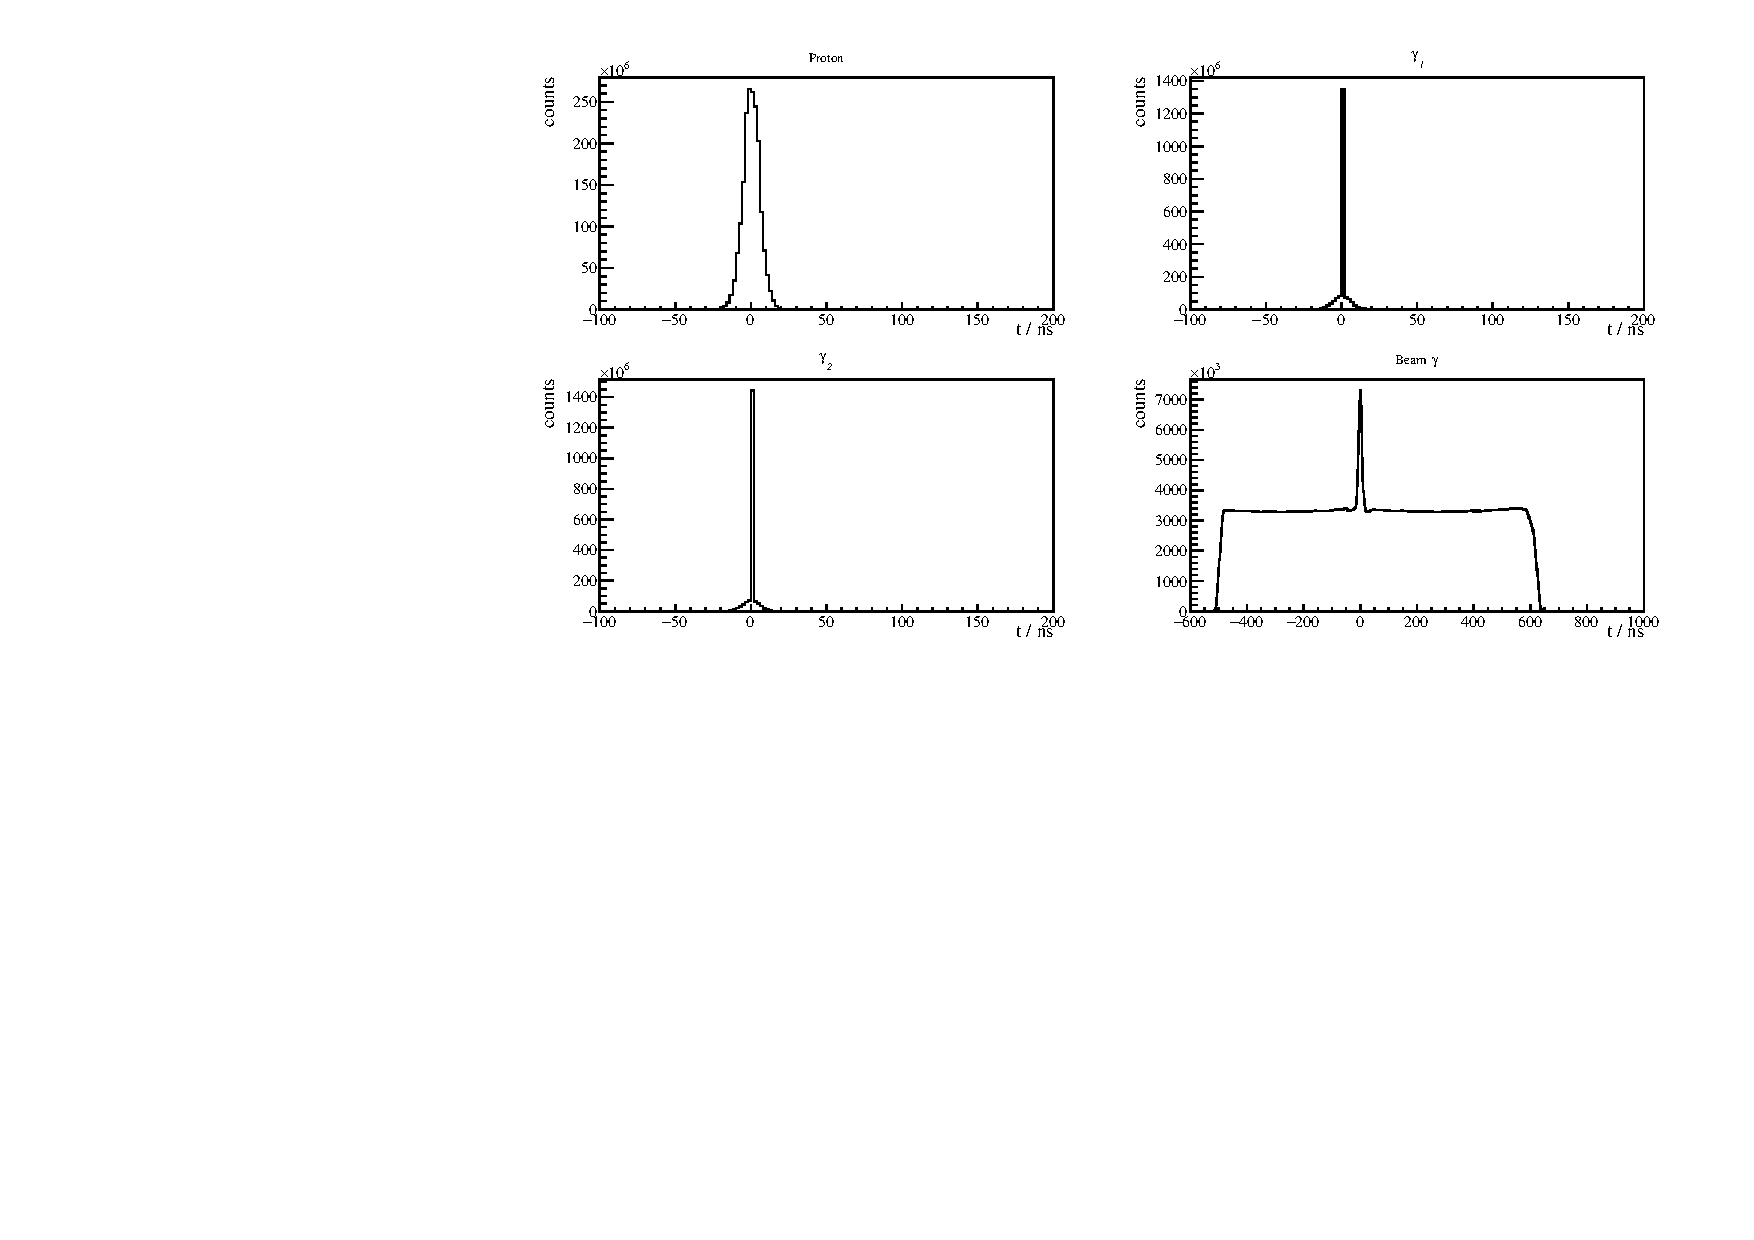
\includegraphics[width=\linewidth]{../figs/hydrogen/time/times.pdf}
	\caption{Time information of all final state particles and the beam photon for 3PED $\eta'$ production}
	\label{fig:time}
\end{figure} 
In all cases prompt peaks centered around \SI{0}{\nano\s} (the trigger time) are visible. Since the final state photons move with velocity $c$ their timing information does not underlie fluctuations, as is the case for the final state proton on the contrary. The tagged, uncorrelated beam photons are visible as flat background underneath the prompt peak in the time of the beam photon. Naturally, only coincident events may be referred to  as $\eta'$ candidates for the further analysis and thus only events with time information of at least one final state particle are kept. Photons need to be detected in the MiniTAPS or forward
detector to acquire time information. To determine coincidence it is convenient to define the \emph{reaction time} 
\begin{equation}
	t_\text{reaction}=\begin{cases}
		t_\text{beam}-t_\text{meson} & \text{ meson time exists}\\
		t_\text{beam}-t_\text{recoil} & \text{ meson time does not exist},
	\end{cases}
\end{equation}
where the meson time $t_\text{meson}$ is appointed either the averaged time of both decay photons or the time of a single photon if only one photon has time information. $t_\text{beam}$ and $t_\text{recoil}$ are the time of the beam photon and recoil proton, respectively. Figure \ref{fig:time_r} shows the reaction time for 2.5PED and 3PED events; a clear prompt peak centred at 0 is visible, the colored area indicates the chosen range of $t_\text{reaction}\in[-8,5]\si{\nano\s}$. However, this cut still contains random time background underneath the prompt peak. This may be accounted for by \emph{sideband substraction}, assuming the background is flat. All events residing in the prompt peak with $t_r\in[-8,5]\si{\nano\s}$ will be assigned a weight of $w_p=+1$ while sideband events with $t_r\in[-200,-100]\si{\nano\s}\lor t_r\in[100,200]\si{\nano\s}$ will be assigned a weight of $w_s=-\frac{13}{200}$. Any histogram $N$ that is filled in the following will then consist of prompt peak events $N_\text{prompt}$ and sideband events $N_\text{sideband}$ $$N=N_\text{prompt}+w_s\cdot N_\text{sideband},$$ such that the random time background underneath the prompt peak is substracted. In addition, the time difference between meson and proton and between the two photons is demanded to be within $[-10,10]\si{\nano\s}$. All described cuts to the data, including the sideband substraction are referred to as the \emph{time cut} in the following.

\begin{figure}[htbp]
	\centering
	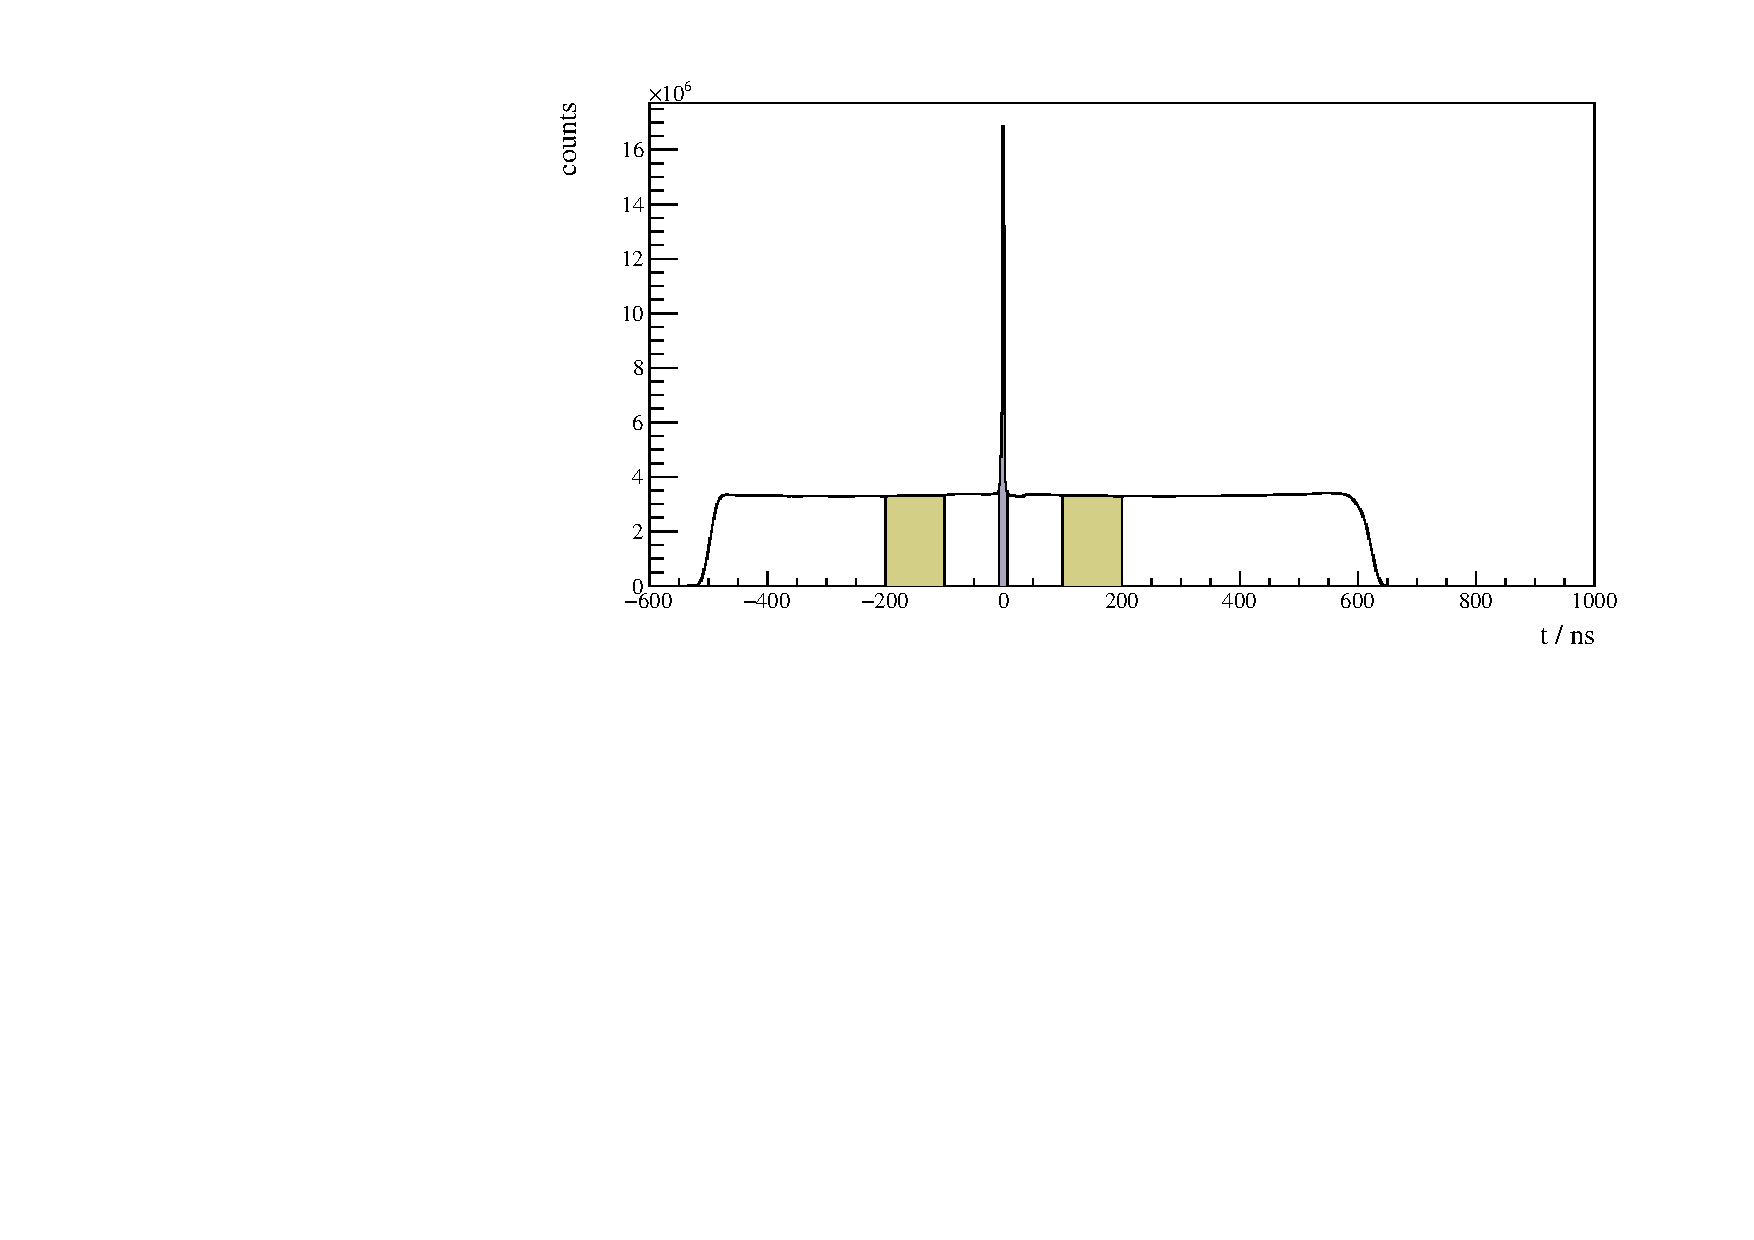
\includegraphics[width=\linewidth]{../figs/hydrogen/time/reaction_time.pdf}
	\caption{Reaction time $t_r$ for 3PED $\eta'$ production}
	\label{fig:time_r}
\end{figure} 

\section{Kinematic constraints}
After charge and time cut, additional cuts can be derived from energy and momentum conservation. Let $p_\text{beam}$ and $p_p$ be the four momenta of the initial state beam photon and proton, respectively. Then \begin{equation}
	p_\text{beam}+p_p=p_\text{recoil}+p_\text{meson}
\end{equation}
holds, with $p_\text{recoil}$ being the momentum of the recoiling proton and $p_\text{meson}$ the meson momentum.
\subsection{Coplanarity}
In the initial state there is vanishing transversal momentum $p_{xy}$ since the target protons are at rest and the beam photon impinges in $z$-direction. Naturally this transversal momentum has to vanish in the final state as well, such that \begin{equation}
	\mathcal{P}_{xy} \left[p_\text{recoil}+p_\text{meson}\right]=0,
	\label{eq:copl}
\end{equation}
where $\mathcal{P}_{xy}$ is the projection operator to the transversal plane. Equation \eqref{eq:copl} is valid if and only if meson and proton lie back to back (coplanar) in the $x$-$y$ plane, which is quantified by the difference of their azimuthal angles $\phi_\text{meson}$ and $\phi_\text{recoil}$ being $\SI{180}{\degree}$
\begin{equation}
	\left|\phi_\text{meson}-\phi_\text{recoil}\right|\overset{!}{=}\SI{180}{\degree}.
\end{equation}